\documentclass[11pt]{scrartcl}
\usepackage[sexy]{evan}
\usepackage{graphicx}

\newcommand{\N}{\mathbb{N}}
\newcommand{\Z}{\mathbb{Z}}
\newcommand{\F}{\mathbb{F}}
\newcommand{\Q}{\mathbb{Q}}
\newcommand{\R}{\mathbb{R}}
\newcommand{\C}{\mathbb C}


\newcommand{\Vu}{\mathbf{u}}
\newcommand{\Vv}{\mathbf{v}}
\newcommand{\Vw}{\mathbf{w}}
\newcommand{\Vx}{\mathbf{x}}
\newcommand{\Ve}{\mathbf{e}}
\newcommand{\Vc}{\mathbf{c}}
\newcommand{\Vb}{\mathbf{b}}



\newcommand{\Va}{\mathbf{a}}

\newcommand{\Vhx}{\mathbf{\hat{x}}}

\newcommand{\Vy}{\mathbf{y}}
\newcommand{\Vz}{\mathbf{z}}
\newcommand{\Vo}{\mathbf{0}}

%From Topology
\newcommand{\cT}{\mathcal{T}}
\newcommand{\cB}{\mathcal{B}}
\newcommand{\cC}{\mathcal{C}}

\usepackage{answers}
\Newassociation{hint}{hintitem}{all-hints}
\renewcommand{\solutionextension}{out}
\renewenvironment{hintitem}[1]{\item[\bfseries #1.]}{}
\declaretheorem[style=thmbluebox,name={Theorem}]{thm}

\begin{document}
\title{CS 189}
\author{Vishal Raman}
\thispagestyle{empty}
$ $
\vfill
\begin{center}

\centerline{\huge \textbf{CS 189 Lecture Notes, Fall 2020}}
\centerline{\Large \textbf{Machine Learning} } 
\centerline{Professor: Anant Sahai, Jennifer Listgarten, Jitendra Malik}
\centerline{Vishal Raman}
\end{center}
\vfill
$ $
\newpage
\thispagestyle{empty}
\tableofcontents
\newpage
%\maketitle
\section{August 31th, 2020}
\subsection{Basics}
We would like to understand patterns from data, which means being able to predict.  If a pattern exists, it will be confirmed with prediction, to some extent.

\begin{definition}[Supervised Learning] We have data $\Vx_i$, outputs $y_i$. We have a success if given $\Vx$, not in our data, we can predict $\hat{y}$ which is "correct".
\end{definition}

There are two kinds of outputs we can consider:
\begin{itemize}
\item Continuous scalars of vectors, which are real or complex valued.  We consider problems of this form "regression problems".
\item Categorical "quantities", ex. "dog" vs "cat" vs "banana".  We consider problems of this form "classification problems".  We immediately have the problem of representation for categorical variables.
\end{itemize}

The usual solution is as follows:
\begin{definition}[One-hot Encoding] We encode a categorical variable as a vector, where entries correspond to boolean variables on the categories.   In the case of binary variables, it suffices to take $y = \pm 1$, for each category.
\end{definition}
\begin{example} $\hat{y} = [1, 0, 0]$ corresponds to Dog, Not Cat, Not Banana.  
\end{example}

Question: Can all problems be reduced to regression?

Answer:  It turns out that regression-type problems can be mended as optimization problems.  For this reason, we try to cast ML as optimization problems, which will sometimes have a regression-type feeling to them.

The levels of an ML problem:
\begin{enumerate}
\item Problem: We have data(a collection of $(x_i, y_i)$ pairs) and want to predict $\hat{y}$ with $x_i$.
\item Model: what kind of pattern are we looking for?  (finding all possible patterns is impossibly difficult)
\item Approach: a learning algorithm, which is done by framing and solving an Optimization problem.
\end{enumerate}

\begin{definition}[Least-Squares Problem] Find $\Vw$ that minimizes $\|A\Vw - \Vb\|^2$.
\end{definition}

\begin{example} We would like to predict the orbit of Cerus.  Problem: We have take $(x, y)$ pairs in the plane.  
Model: Find an elliptical orbit for Cerus.  
\end{example}
We model the problem as a Least-Squares problem. We have points $(x_1, y_1), (x_2, y_2), \dots, (x_n, y_n)$.  Any conic section is of the form $w[0]x^2 + w[1]y^2 + w[2]xy + w[3]x + w[4]y + w[5] = 1$ (this is a somewhat relaxed approach to the problem, but it is easy to implement).

We find $\text{arg}\min_{\Vw} \| [x_i^2, y_i^2, x_iy_i, x_i, y_i, 1]\Vw - [\mathbf{1}]\|^2$.   We call the $x_i^2, y_i^2, x_iy_i, x_i, y_i$ features.

\subsection{Features}
\begin{definition}[Features] The components of the pattern that we are trying to learn.  It is a mapping from the input data.
\end{definition}
Picking the features is where ML is more an art than a science, and usually requires domain knowledge to be successful.
\begin{definition}[Linear Regression] The desired pattern, a linear combination of features.
\end{definition}
\subsection{Classification Comments}
\begin{definition}[Signature Approach] Every class $\ell$ is associated to a signature $\Vw_\ell$.  Given features $\Vx$, we compute $\text{arg}\max_{\ell} \Vx^T \Vw_\ell$.
\end{definition}
The learning problem is to find the $\Vw_\ell$.  For the binary case, with two signatures, we wish to check $\Vx^T \Vw_1 > \Vx^T\Vw_2\Rightarrow \Vx^T(\Vw_1 - \Vw_2) > 0$, so it reduces to a single signature.

We can learn the $\Vw_\ell$ using one-hot-encoding to set $\Vy$.  
%include graphics
\begin{center}
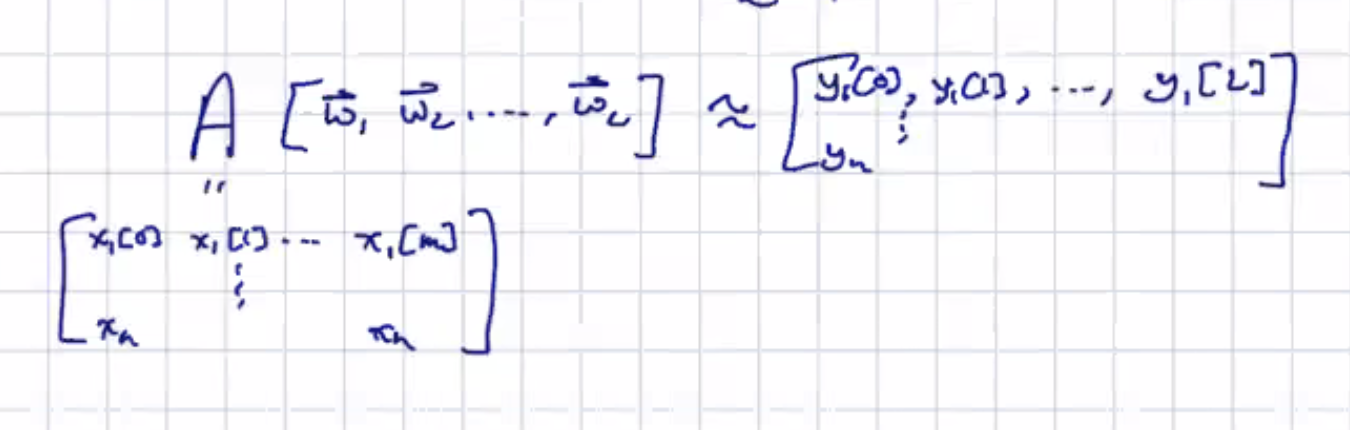
\includegraphics[scale = 0.5]{matrixMultiply.png}
\end{center}
It suffices to take $\hat{w} = (A^TA)^{-1}A^TY$.


Where do features come from?
\begin{itemize}
\item Domain-specific knowledge
\item Universal Function Approximation: any function on a compact set can be approximated to any chosen accuracy.
\end{itemize}
\subsection{Conditioning and Ridge Regularization}
What can go wrong with squared-error approaches?  The first clear problem is that $A^TA$ might not be invertible.

We take an SVD approach to $(A^TA)^{-1}A^T$: let $A = U\Sigma V^T$.
\begin{center}
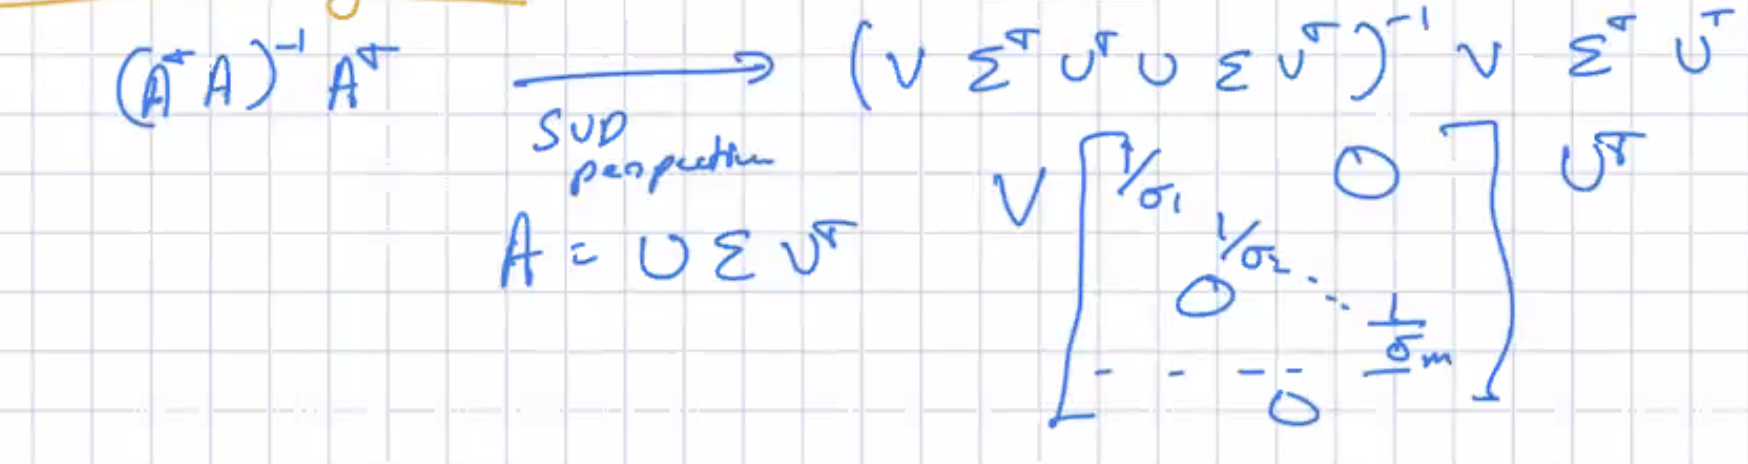
\includegraphics[scale=0.5]{svd.png}
\end{center}
Notice that we have reciprocals of singular values, which will blow up for small values.  This is a problem because the noise in the data will be amplified by very large values. 

 We could take a dimensionality reduction(PCA) approach to kill off small singular values, or we take a hack: compute $(A^TA + \lambda I)^{-1}A^T$.  We now have $\hat{w}  = (A^TA + \lambda I)^{-1}A^T Y$.  We note that 
$$\frac{\sigma_j}{\sigma_j^2 + \lambda} = \frac{1}{\sigma_j}\left (\frac{1}{1 + \frac{\lambda}{\sigma_j^2}}\right)$$
which acts as a high-pass filter.  This is known as "ridge regularization".
\newpage
\section{September 2nd, 2020}
\subsection{Universal Function Approximation and Features}
Recall, we have the goal of going from inputs, $\Vx \in \R^r$ , to predictions, $\hat{y}$.  We consider scalar $y$(we discussed the case of vector $y$ in the previous lecture).  

We use a linear parameterization of the patterns we want to learn:
$$y = \sum_{i=1}^{m-1} w[i]\phi_i(\Vx)$$
where $\phi_i$ is the $i$-th feature and $\Vw \in \R^m$.
The feature vector is denoted $\mathbf{\phi} = \begin{bmatrix}
\phi_0 \\ \phi_1 \\ \dots \\ \phi_{m-1}
\end{bmatrix}$

The map $$\Vx \mapsto \mathbf{\phi}(\Vx),$$
is called a \textbf{lifting} if $m > r$ and a \textbf{distillation} if $m < r$.

\begin{definition}[Universal Feature Family] Families that allow (with enough features) arbitrarily good approximations of target patterns.
\end{definition}
Some examples include:
\begin{itemize}
\item Polynomials,
\item Fourier Features,
\item Piecewise Linear functions.
\end{itemize}
\begin{example}[Feature Growth]  We have the following classes of polynomials.

\begin{itemize}
\item \textbf{Univariate}: $1, x, x^2, x^3, x^4, \dots, x^d$ which requires $d+1$ features.
\item \textbf{Bivariate}: $1, x_1, x_2, x_1^2, x_1x_2, x_2^2, \dots$
\item \textbf{Trivariate}: $1, x_1, x_2, x_3, x_1^2, x_1x_2, x_1x_3, x_2x_3, x_2^2, x_3^2, \dots$
\end{itemize}
You can see that there are $\binom{r+d}{r} =\binom{r+d}{d}$ order at-most-$d$ monomials in $r$ variables(consider a stars-and-bars argument).  This grows on the order $d^r$ if $r$ is fixed, $r^d$ is $d$ is fixed, or $2^{dH(\frac{r}{d+r})}$ if $r$ is a proportion of $d$.  We see that the number of polynomial features grow with exponential order.

We saw last time that we would like to turn problems into optimization, $\min \| A\Vw - \Vb\|^2 : (A^TA)^{-1}A\Vb$. We have 
$$A = \begin{bmatrix}
\phi_1(x_1) & \phi_2(x_1) & \dots & \phi_m(x_1) \\
\phi_1(x_2) & \phi_2(x_2) & \dots & \phi_m(x_2) \\
\vdots & \vdots & \ddots & \vdots \\
\phi_1(x_n) & \phi_2(x_n) & \dots & \phi_m(x_n) \\
\end{bmatrix}.$$
This has dimension $n$ by $m$.  When $m > n$, $A^TA$ is $m$ by $m$, so it is singular.
\end{example}
\subsection{Ridge Regression}
Last time, we were considering $(A^TA)^{-1}A^T$ in the SVD sense, with $A = U \Sigma V^T$.  We had a "hack":  consider $(A^TA + \lambda I)^{-1}$ instead, which is well defined.  On the diagonal, we had values 
$$\frac{\sigma_j}{\sigma_j^2 + \lambda} = \frac{1}{\sigma_j}\left (\frac{1}{1 + \frac{\lambda}{\sigma_j^2}}\right).$$
We noticed that this behaves like a "highpass filter".
\begin{center}
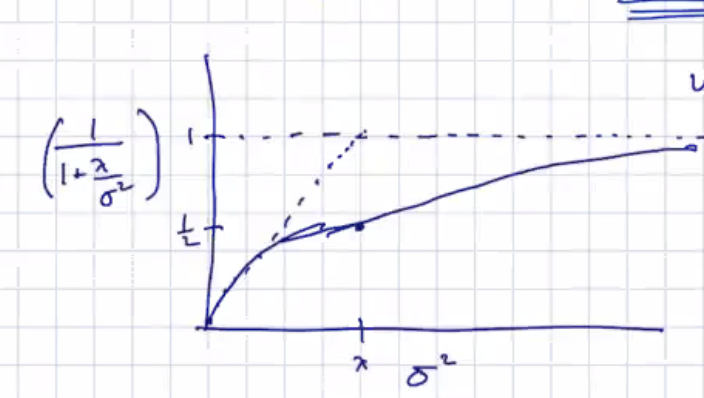
\includegraphics[scale=0.5]{graph.png}
\end{center}
$$\frac{1}{1 + \frac{\lambda}{\sigma^2}} \approx \begin{cases}
\frac{\sigma^2}{\lambda} & \text{ if } \sigma^2 << \lambda \\ 
1 & \text{ if } \sigma^2 >> \lambda 
\end{cases}$$
When $\sigma_j^2 << k$, then $$\frac{\sigma_j}{\sigma_j^2 + \lambda} \approx \frac{1}{\sigma_j}\left (\frac{\sigma_j^2}{\lambda}\right ) = \frac{\sigma_j}{\lambda}.$$

Ridge regression is a soft way of expression trust is only those directions $\Vv_j$ in the parameter space that have large enough $\sigma_j$.  Alternatively, ridge regression doesn't trust variations in $\Vy$ along $\Vu_j$(from SVD, associated with the output) with small $\sigma_j$.

We are left with the question: how to we choose $\lambda$?

\begin{example} Suppose $$\Vy = A \Vw_{true} = U\Sigma V^T \Vw_{true} = \sum_{i} \Vu_i \sigma_i \Vv_i^T \Vw_{true}.$$ 

Suppose we have $\hat{w} = (A^TA + \lambda I)^{-1} A^T \Vy = \sum_i v_i \frac{\sigma_i}{\sigma_i^2 + \lambda}u_i^T \Vy$.  Instead of getting $\Vv_i^T\Vw_{true}$, what do we get?

$$\hat{w} = \frac{\sigma_i}{\sigma_i^2 + \lambda} \Vv_i \sigma_i \Vu_i^T \Vw_{true} = \frac{\sigma_i^2}{\sigma_i^2 + \lambda} \Vv_i\Vu_i^T \Vw_{true},$$
and note that 
$$ \frac{\sigma_i^2}{\sigma_i^2 + \lambda} = \begin{cases}
1 & \text{ if } \sigma_i^2 >> \lambda \\ 
0 & \text{ if } \sigma_i^2 << \lambda 
\end{cases}.$$
We see that we pick $\lambda$ so that it is smaller than $\sigma_i^2$ for directions we trust and larger than $\sigma_i^2$ for directions we don't trust.
\end{example}

To what optimization problem in $(A^TA + \lambda I)^{-1} A^T b$ the answer? We know that $(A^TA)^{-1}A^Tb$ optimizes $\text{arg}\min\|Aw - b\|^2$, so what does ridge regression optimize?

We will show that it optimizes 
$$\text{arg}\min \|Aw -b \|^2 + \lambda \|w\|^2.$$

Note that 
\begin{align*}
 (Aw-b)^T(Aw-b) + \lambda w^T w &= w^TA^TAw - b^TAw - w^TA^Tb + b^Tb + \lambda w^Tw \\
 &= w^T(A^TA + \lambda I)w - 2b^TAw + b^Tb.
\end{align*}
We take the derivative $\frac{d}{dw}$ to get 
$$-2b^TA + w^T(A^TA + \lambda I) + w^T(A^TA + \lambda I)^T = 2w^T(A^TA + \lambda I) - 2b^TA = 0^T.$$
Hence,
$$w^T = b^TA(a^TA + \lambda I)^{-1} \Rightarrow w = (A^TA + \lambda I)^{-1}A^Tb.$$ 

\subsection{Hyperparameters}
Consider the plot of $\|A\hat{w} - b\|^2$ as a function of $\lambda$.
\begin{center}
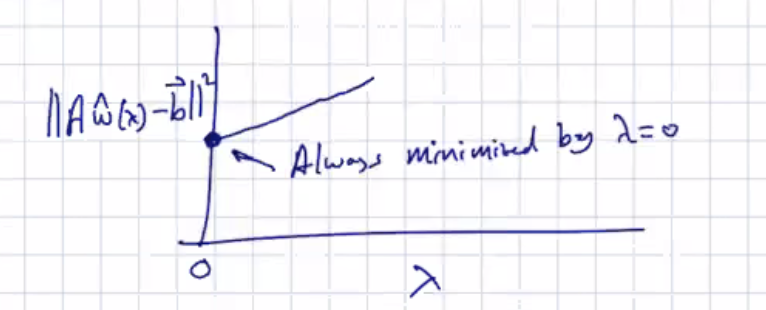
\includegraphics[scale=0.75]{lambda.png}
\end{center}
We would always want $\lambda = 0$ given the training data.  $\lambda$ is a hyperparameter, where if we tried to optimize it, we would always get $0$.
\pagebreak
\section{September 9th, 2020}
\subsection{Test Sets}
\subsection{Validation and Hyper-parameters}
\subsection{K-fold Cross-Validation}
\subsection{Probability and Toy Models}

\end{document}
